\documentclass[english,notitlepage]{revtex4-1}  % defines the basic parameters of the document
%For preview: skriv i terminal: latexmk -pdf -pvc filnavn



% if you want a single-column, remove reprint

% allows special characters (including æøå)
\usepackage[utf8]{inputenc}
%\usepackage[english]{babel}

%% note that you may need to download some of these packages manually, it depends on your setup.
%% I recommend downloading TeXMaker, because it includes a large library of the most common packages.

\usepackage{physics,amssymb}  % mathematical symbols (physics imports amsmath)
\include{amsmath}
\usepackage{graphicx}         % include graphics such as plots
\usepackage{xcolor}           % set colors
\usepackage{hyperref}         % automagic cross-referencing (this is GODLIKE)
\usepackage{listings}         % display code
\usepackage{subfigure}        % imports a lot of cool and useful figure commands
\usepackage{float}
%\usepackage[section]{placeins}
\usepackage{algorithm}
\usepackage[noend]{algpseudocode}
\usepackage{subfigure}
\usepackage{tikz}
\usetikzlibrary{quantikz}
% defines the color of hyperref objects
% Blending two colors:  blue!80!black  =  80% blue and 20% black
\hypersetup{ % this is just my personal choice, feel free to change things
    colorlinks,
    linkcolor={red!50!black},
    citecolor={blue!50!black},
    urlcolor={blue!80!black}}

%% Defines the style of the programming listing
%% This is actually my personal template, go ahead and change stuff if you want



%% USEFUL LINKS:
%%
%%   UiO LaTeX guides:        https://www.mn.uio.no/ifi/tjenester/it/hjelp/latex/
%%   mathematics:             https://en.wikibooks.org/wiki/LaTeX/Mathematics

%%   PHYSICS !                https://mirror.hmc.edu/ctan/macros/latex/contrib/physics/physics.pdf

%%   the basics of Tikz:       https://en.wikibooks.org/wiki/LaTeX/PGF/Tikz
%%   all the colors!:          https://en.wikibooks.org/wiki/LaTeX/Colors
%%   how to draw tables:       https://en.wikibooks.org/wiki/LaTeX/Tables
%%   code listing styles:      https://en.wikibooks.org/wiki/LaTeX/Source_Code_Listings
%%   \includegraphics          https://en.wikibooks.org/wiki/LaTeX/Importing_Graphics
%%   learn more about figures  https://en.wikibooks.org/wiki/LaTeX/Floats,_Figures_and_Captions
%%   automagic bibliography:   https://en.wikibooks.org/wiki/LaTeX/Bibliography_Management  (this one is kinda difficult the first time)
%%   REVTeX Guide:             http://www.physics.csbsju.edu/370/papers/Journal_Style_Manuals/auguide4-1.pdf
%%
%%   (this document is of class "revtex4-1", the REVTeX Guide explains how the class works)


%% CREATING THE .pdf FILE USING LINUX IN THE TERMINAL
%%
%% [terminal]$ pdflatex template.tex
%%
%% Run the command twice, always.
%% If you want to use \footnote, you need to run these commands (IN THIS SPECIFIC ORDER)
%%
%% [terminal]$ pdflatex template.tex
%% [terminal]$ bibtex template
%% [terminal]$ pdflatex template.tex
%% [terminal]$ pdflatex template.tex
%%
%% Don't ask me why, I don't know.

\begin{document}

\title{Project 1 - FYS3150}               % self-explanatory
\author{Josef Ayman M.}                      % self-explanatory
\date{\today}                             % self-explanatory
\noaffiliation                            % ignore this, but keep it.


\maketitle

\textit{
    \href{https://github.uio.no/josefam/FYS3150}{github.uio.no/josefam/FYS3150}
}

\section*{Problem 1}
We check that $u(x) = 1 - (1 - e^{-10}) x - e^{-10 x}$ is an exact solution to our Poisson equation.

We simplify it:

\[
    u(x) = 1-x+e^{-10}x-e^{-10x}
\]

Then we try to find the second derivative:

\[
    u'(x)=-1+e^{-10}+10e^{-10x} \\
    u''(x) =-100e^{-10x}
\]


Which when fits the source term $-(-100e^{-10x}) = f(x) = 100e^{-10x}$

And the boundary conditions:

\[
    u(0)=1-0+0-1=0 \\
    u(1)=1-1+e^{-10}-e^{-10}=0
\]

\section*{Problem 2}
In problem 2 we will write a program that:

\begin{itemize}
    \item Defines a vector of $x$ values.
    \item Evaluates the exact solution at each point.
    \item Writes the results to a file.
    \item It's recommended to use the \textit{\href{https://arma.sourceforge.net/}{armadillo}} library.
\end{itemize}

As we can see in \figurename{ \ref{fig:poisson_exact}}, the exact solution to the Poisson equation is a curve that starts at 1 and decreases to 0 as $x$ approaches 1.

\begin{figure}%[h!]
    \centering %Centers the figure
    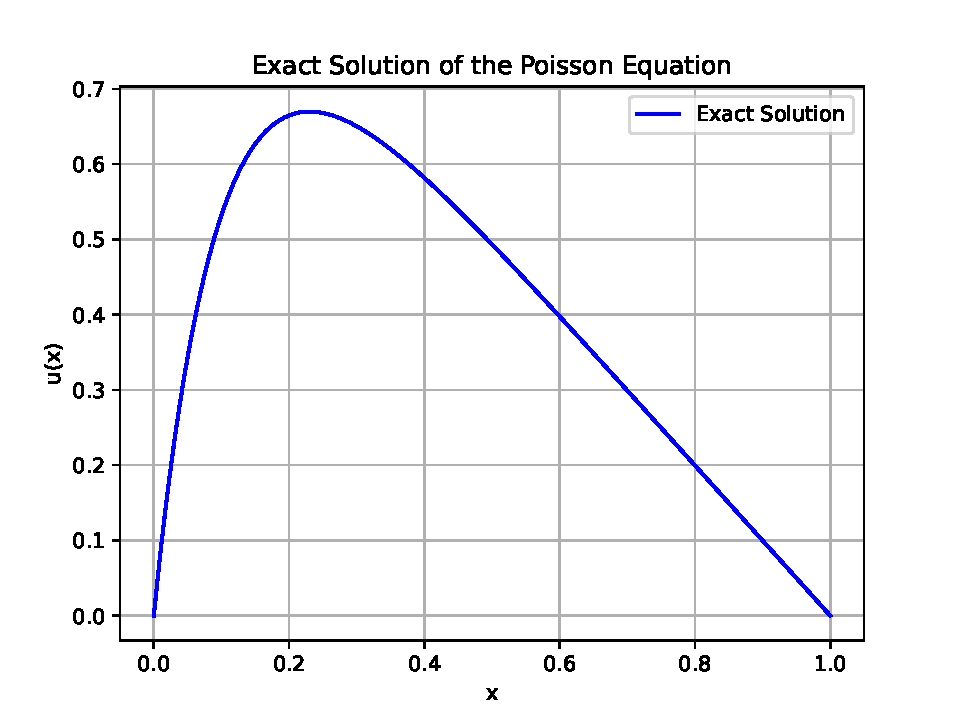
\includegraphics[scale=0.75]{problem2/poisson_solution_plot.pdf} %Imports the figure.
    \caption{Plot of the exact solution to the Poisson equation.} %Short caption for the figure.
    \label{fig:poisson_exact} %Label for referencing in the text.
\end{figure}

\section*{Problem 3}
\textbf{Discretization of the Domain}

\begin{itemize}
    \item The domain $x$ ranges from 0 to 1.
    \item We divide the domain into $N$ equally spaced intervals, where $h$ is the spacing between grid points, $h = \frac{1}{N}$.
    \item Define grid points $x_i$ as:
          $$ x_i = i h \quad \text{for} \; i = 0, 1, 2, \ldots, N $$
\end{itemize}

Let $v_i$ be the approximation to $u(x_i)$.

To approximate the second derivative $\frac{d^2 u}{dx^2}$ at a point $x_i$, we use the \textbf{finite difference method}. The central difference approximation for the second derivative is:

$$
    \frac{d^2 u}{dx^2} \approx \frac{u(x_{i+1}) - 2 u(x_i) + u(x_{i-1})}{h^2}
$$

\textbf{Substitute into the Poisson Equation}

$$
    -\frac{u(x_{i+1}) - 2 u(x_i) + u(x_{i-1})}{h^2} = f(x_i)
$$

\textbf{Simplify}

Rearrange the equation to solve for the discrete approximation:

$$
    v_{i+1} - 2 v_i + v_{i-1} = -h^2 f_i
$$

or

\begin{equation}{\label{eq:discrete_poisson}}
    -\frac{v_{i+1} - 2 v_i + v_{i-1}}{h^2} = f_i
\end{equation}

\textbf{Boundary Conditions}

In the problem, the boundary conditions are $u(0) = 0$ and $u(1) = 0$. Therefore:

$$
    v_0 = 0 \\v_N = 0
$$

Putting it all together, the discretized version of the Poisson equation is:

$$
    v_{i+1} - 2 v_i + v_{i-1} = -h^2 \cdot 100 e^{-10 x_i}
$$

for $i = 1, 2, \ldots, N-1$, with boundary conditions:

$$
    v_0 = 0 \quad \text{and} \quad v_N = 0
$$

\section*{Problem 4}
To rewrite the discretized Poisson equation as a matrix equation,
we start from the discretized second derivative equation \ref{eq:discrete_poisson}:

This can be written in matrix form as $\mathbf{A} \vec{v} = \vec{g}$, where  $\mathbf{A}$ looks like:

$$
    \mathbf{A} = \begin{bmatrix}
        2  & -1 & 0  & 0  \\
        -1 & 2  & -1 & 0  \\
        0  & -1 & 2  & -1 \\
        0  & 0  & -1 & 2
    \end{bmatrix}
$$

$g_i$ is our right hand of the equation.

$$
    \begin{bmatrix}
        2  & -1 & 0  & 0  \\
        -1 & 2  & -1 & 0  \\
        0  & -1 & 2  & -1 \\
        0  & 0  & -1 & 2
    \end{bmatrix}
    \begin{bmatrix}
        v_1 \\
        v_2 \\
        v_3 \\
        v_4
    \end{bmatrix} = \begin{bmatrix}
        g_1 \\
        g_2 \\
        g_3 \\
        g_4
    \end{bmatrix}
$$

$$
    \begin{bmatrix}
        2v_1 & -v_2 & 0    & 0    \\
        -v_1 & 2v_2 & -v_3 & 0    \\
        0    & -v_2 & 2v_3 & -v_4 \\
        0    & 0    & -v_3 & 2v_4
    \end{bmatrix} = \begin{bmatrix}
        g_1 \\
        g_2 \\
        g_3 \\
        g_4
    \end{bmatrix}
$$

We now showed that we can rewrite the equation in the matrix form $\mathbf{A} \vec{v} = \vec{g}$

\section*{Problem 5}
\subsection*{Problem a}
The matrix equation for the internal points can be written as:

$$
    \mathbf{A} \vec{v} = \vec{g}
$$

$$
    \mathbf{A} = \begin{bmatrix}
        2      & -1     & 0      & \cdots & 0      \\
        -1     & 2      & -1     & \cdots & 0      \\
        \vdots & \ddots & \ddots & \ddots & \vdots \\
        0      & \cdots & -1     & 2      & -1     \\
        0      & \cdots & 0      & -1     & 2
    \end{bmatrix}, \quad \vec{v} = \begin{bmatrix}
        v_1    \\
        v_2    \\
        \vdots \\
        v_n
    \end{bmatrix}, \quad \vec{g} = \begin{bmatrix}
        g_1    \\
        g_2    \\
        \vdots \\
        g_n
    \end{bmatrix}
$$

Writing out the first and last rows, we see that:

$$
    2 v_1 - v_2 = g_1, \quad -v_{n-1} + 2 v_n = g_n
$$

These correspond to the internal points of $\vec{v}^*$, excluding the boundary values. Since  $v_1$ corresponds to the second element of $\vec{v}^*$and  $v_n$ corresponds to the second-to-last element, we conclude that $m = n + 2$, accounting for the two boundary conditions $v^*_1 = 0$ *and $v^*_m = 0$*.

\subsection*{Problem b}
The vector $\vec{v}$, which we solve for in $\mathbf{A} \vec{v} = \vec{g}$, represents the internal points of \( \vec{v}^* \). The boundary points $v^*_1 = 0$ and $ v^m = 0 $ are known and are excluded from the matrix equation. Additionally, $g_i$ corresponds to $f(x{i+1})$, where $x_{i+1}$ is the corresponding discretized point.

\section*{Problem 6}

\subsection*{Problem a - Algorithm for Solving the System}{\label{sec:algorithm}}

To solve the system \( \mathbf{A} \vec{v} = \vec{g} \) where \( \mathbf{A} \) is a general tridiagonal matrix,
we can use a method called \textit{\href{https://en.wikipedia.org/wiki/Tridiagonal_matrix_algorithm}{Thomas Algorithm}}
(a specialized form of Gaussian elimination for tridiagonal matrices).


Here's the algorithm broken down step by step:

\begin{algorithm}[H]
    \caption{Thomas Algorithm for Tridiagonal Matrices}
    \begin{algorithmic}[1]
        \State \( c_1 \gets \frac{c_1}{b_1} \)
        \State \( g_1 \gets \frac{g_1}{b_1} \)
        \For{\( i = 2 \) to \( n \)}
        \State \( b_i \gets b_i - a_i c_{i-1} \) \Comment{Update diagonal}
        \If{i $<$ n}
        \State \( c_i \gets \frac{c_i}{b_i} \) \Comment{Update superdiagonal (except for the last row)}
        \EndIf
        \State \( g_i \gets \frac{g_i - a_i g_{i-1}}{b_i} \) \Comment{Update right-hand side}
        \EndFor
        \State \( v_n \gets g_n \) \Comment{Backward substitution starts here}
        \For{\( i = n-1 \) to \( 1 \)}
        \State \( v_i \gets g_i - c_i v_{i+1} \) \Comment{Solve for remaining \(v_i\)}
        \EndFor
    \end{algorithmic}
\end{algorithm}

\subsection*{Problem b - Number of Floating-Point Operations (FLOPs)}

We count the number of operations in each phase.

\begin{itemize}
    \item \textbf{Forward substitution:} For each \( i \) from 2 to \( n \), we have 3 FLOPs (2 divisions and 1 subtraction). This gives a total of \( 3(n-1) \) FLOPs.
          \subitem 1 division for \( c_i \)
          \subitem 1 division for  \(g_i\)
          \subitem 1 subtraction for \(b_i\)
    \item \textbf{Backward substitution:} For each \( i \) from \( n-1 \) to 1, we have 2 FLOPs (1 multiplication and 1 subtraction). This gives a total of \( 2(n-1) \) FLOPs.
          \subitem 1 multiplication for \(c_i v_{i+1}\)
          \subitem 1 subtraction for \(g_i - c_i v_{i+1}\)
    \item \textbf{Total:} The total number of FLOPs is \( 3(n-1) + 2(n-1) = 5(n-1) \) = \( 5n - 5 \).
\end{itemize}

\section*{Problem 7}
Here we will write an implementation of the Thomas algorithm we disscussed in
\textbf{Problem 6}.

\begin{figure}%[h!]
    \centering %Centers the figure
    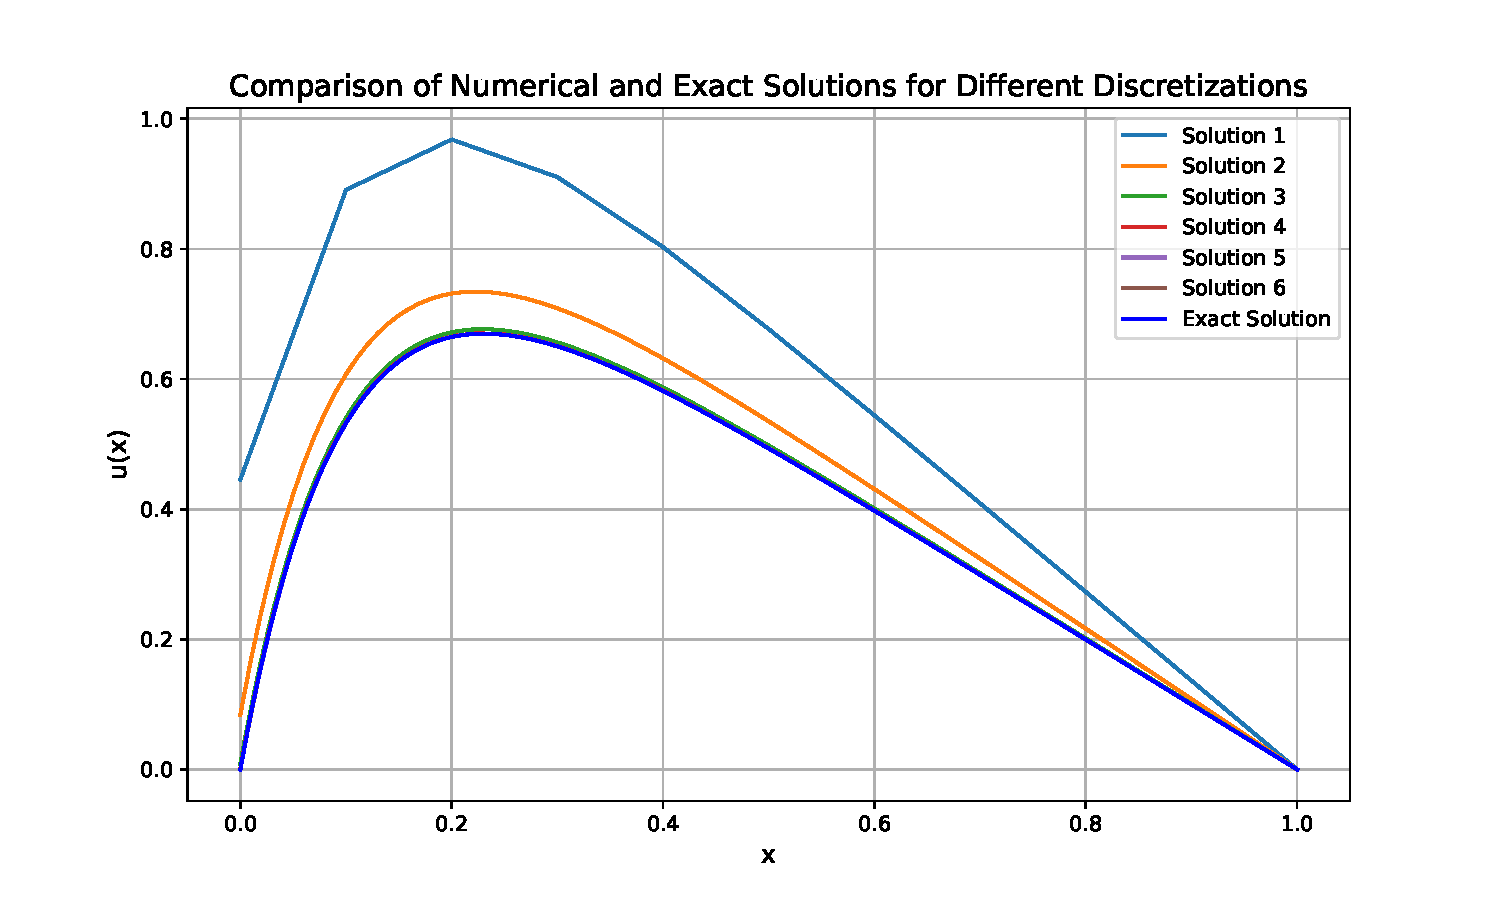
\includegraphics[scale=0.70]{problem7/general_algorithm_plot.pdf} %Imports the figure.
    \caption{Plot of the general algorithm compared to the exact solution.} %Short caption for the figure.
    \label{fig:general_algorithm} %Label for referencing in the text.
\end{figure}

\begin{figure}%[h!]
    \centering %Centers the figure
    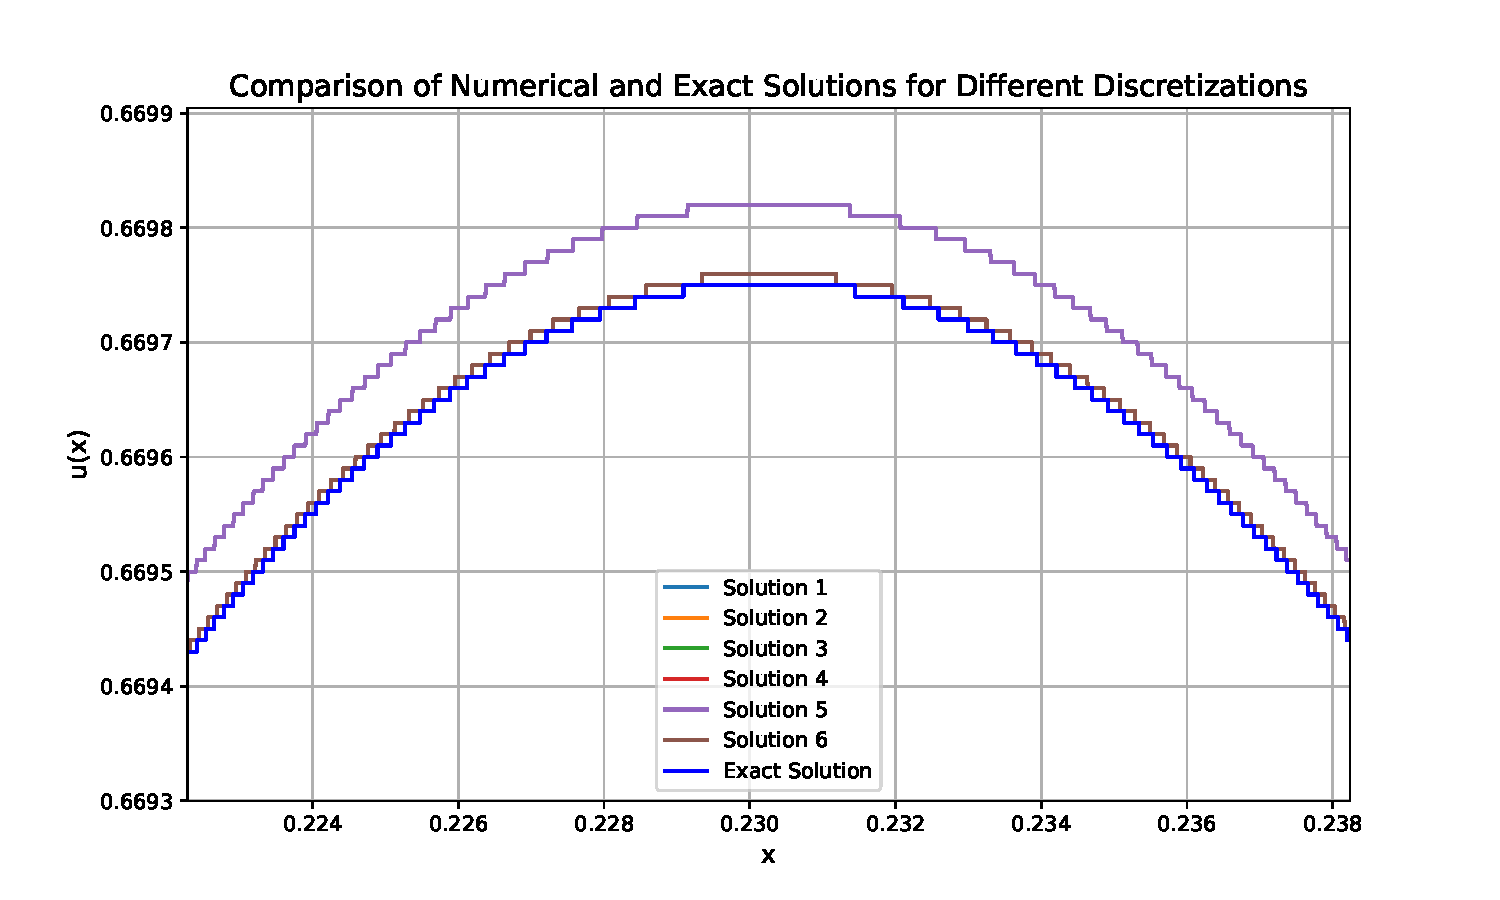
\includegraphics[scale=0.70]{problem7/zoom_in_plot.pdf} %Imports the figure.
    \caption{Zoomed in plot of the general algorithm compared to the exact solution.} %Short caption for the figure.
    \label{fig:general_algorithm_zoomed} %Label for referencing in the text.
\end{figure}

As we can see in \figurename{ \ref{fig:general_algorithm}} and \figurename{ \ref{fig:general_algorithm_zoomed}}, the general algorithm is a good approximation to the exact solution.

\section*{Problem 8}
\subsection*{Problem a - Plotting the Absolute Error}
\figurename{ \ref{fig:absolute_error}} shows the absolute error of the general algorithm compared to the exact solution.

\begin{figure}[h!]
    \centering %Centers the figure
    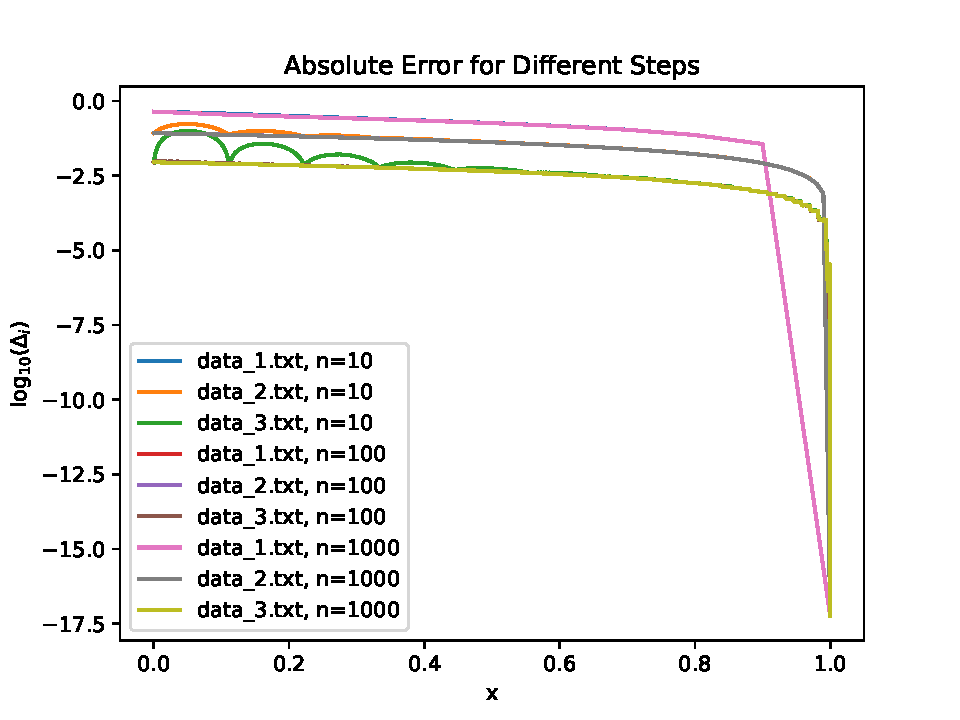
\includegraphics[scale=0.70]{problem8/absolute_error_plot.pdf} %Imports the figure.
    \caption{Plot of the absolute error of the general algorithm compared to the exact solution.} %Short caption for the figure.
    \label{fig:absolute_error} %Label for referencing in the text.
\end{figure}

\subsection*{Problem b - Plotting the Rrelative Error}
\figurename{ \ref{fig:relative_error}} shows the relative error of the general algorithm compared to the exact solution.

\begin{figure}[h!]
    \centering %Centers the figure
    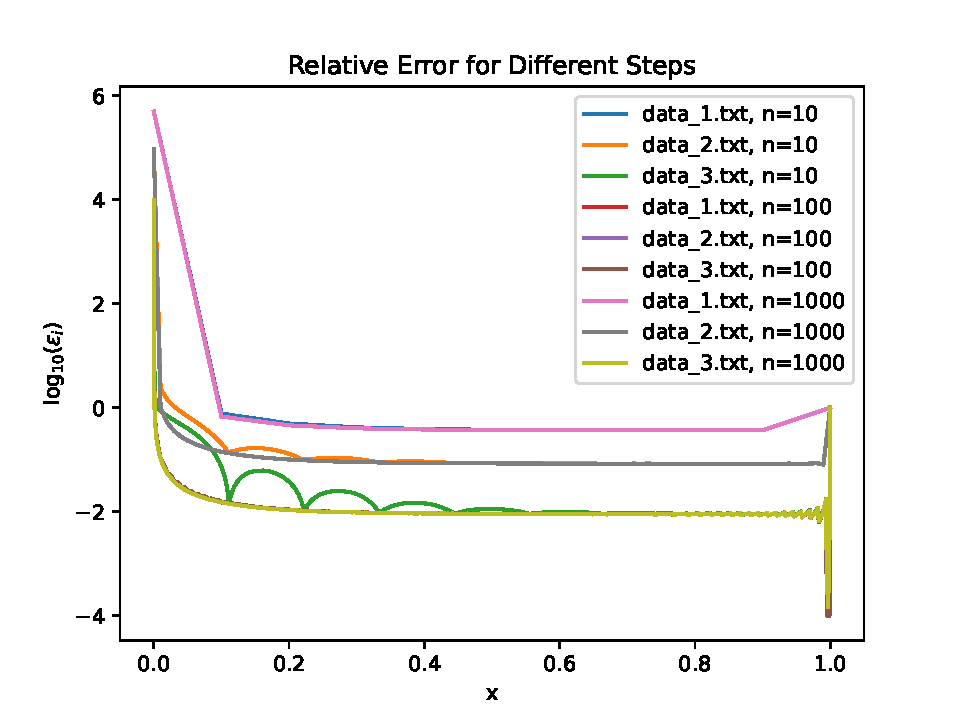
\includegraphics[scale=0.70]{problem8/relative_error_plot.pdf} %Imports the figure.
    \caption{Plot of the relative error of the general algorithm compared to the exact solution.} %Short caption for the figure.
    \label{fig:relative_error} %Label for referencing in the text.
\end{figure}

\subsection*{Problem c - Table of Maximum Relative Error}

Got stuck on this one, and got the same value for all \( N \) values. The value was 494887.

\begin{table*}
    \centering
    \begin{tabular}{|c|c|}
        \hline
        \textbf{N} & \textbf{Max Relative Error} \\
        \hline
        10          & 494887                   \\
        100         & 494887                   \\
        1000        & 494887                   \\
        \hline
    \end{tabular}
    \caption{Table of the maximum relative error for different values of \( N \).}
    \label{tab:relative_error}
\end{table*}

\section*{Problem 9}
\subsection*{Problem a - Specialized Algorithm for the Poisson Equation}
I feel like I already did this in \textbf{Problem 6}.

\section*{Problem 10}

Timing tests:

\begin{table*}
    \centering
    \begin{tabular}{|c|c|}
        \hline
        \textbf{N} & \textbf{Elapsed Time} \\
        \hline
        10          & 1.208e-06 seconds      \\
        100         & 6.375e-06 seconds      \\
        1000        & 6.1125e-05 seconds     \\
        10000       & 0.000607792 seconds    \\
        100000      & 0.00563683 seconds     \\
        1000000     & 0.0485015 seconds      \\
        10000000    & 0.569739 seconds       \\
        \hline
    \end{tabular}
    \caption{Table of the elapsed time for different values of \( N \).}
    \label{tab:elapsed_time}
\end{table*}
\end{document}